\appendix
%\chapter{Online Track Recontruction of TRD for Electron Triggeres}
\chapter{Collision Geometry in Relativistic Heavy Ion Collisions}
\label{app_a_glauber}
Figure~\ref{fig_ap_nncoll} shows the schematic view of the high energy nucleus-nucleus collisions with the impact parameter $b$. 
The geomerical features of the nucleus-nucleus collisions are described by the Glauber model calculation~\cite{bib_glauber}. 
It is widely used to obtain the variables such as $N_{part}$, $N_{coll}$, path length $L$, and the nuclear thickness function $T_{\rm{AA}}$. 
\begin{figure}[!h]
  \centering
  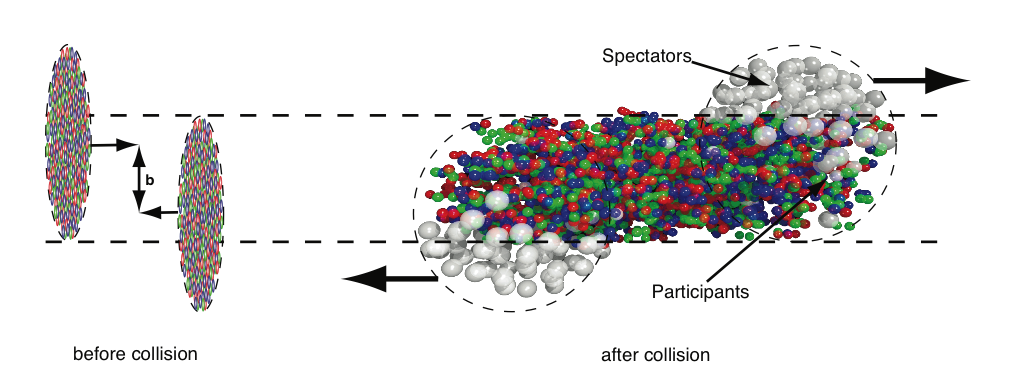
\includegraphics[width=12cm]{app/figure/NN_overview.png}
  \caption{Schematic view of the high energy nucleus-nucleus collisions. The figure is taken from~\cite{bib_nncoll}.}
  \label{fig_ap_nncoll}
\end{figure}

\section{Glauber Model}
In the Glauber model calculation, the density distribution of heavy nuclei is considered by the Woods-Saxon form expressed as 
\begin{equation}
        \rho (r) = \frac{\rho_{0}}{1+e^{(r-R)/d}}
\end{equation}
where $R$ is the radius of necleus, d is called as the skin depth. 

The basic Glauber model requires the following assumption, 
\begin{description}
       \item{-} Nucleons travel to the straigh lines.
       \item{-} Binary nucleon-nucleon collisions are independent each other. 
       \item{-} The inelastic cross section of nucleon-nucleon collisions is same as that in vacuume. 
\end{description}

If we consider the relativistic nucleus-mucleus collisions between A and B with the impact parameter b, 
the participants and the spectators can be defined. 
The participants are nucleons which exist in the overlap region of A and B.
The spectators are defined as the nucleons outside the overlap region of A and B. 

The probability at the transverse position $\bm{s}$ in A is
\begin{equation}
        T_{A}(\bm{s}) = \int \rho_{A} (\bm{s}, z_{A})dz_{A}
\end{equation}
By integrating over the joint probablity in small unit $d^{s}$ is $T_{A}(\bm{s})T_{B}(\bm{s}-\bm{b})$, the effective overlap region is obtained,  
\begin{equation}
        T_{AB}(b) = \int T_{A}(\bm{s})T_{B}(\bm{s}-\bm{b})ds^{2}.
\end{equation}
$T_{AB}(b)$ is defined as the thickness function. 
The probability of occuarance of a nucleon-nucleon collision between A and B is expressed by
\begin{equation}
T_{AB} (\bm{b}) \sigma_{NN} = \int d\bm{b}_{A}dz_{A}\rho_{A}(\bm{b}_{A}, z_{A}) d\bm{b}_{B}dz_{B}\rho_{B}(\bm{b}_{B}, z_{B}) t(\bm{b}-\bm{b}_{A}-\bm{b}_{B})\sigma_{NN},
\end{equation}
where $t(\bm{b})$ is the probability of a nucleon-nucleon collision within the tranverse element $d\bm{b}$.

The probability of having n nucleon-nucleon collisions can be described by the binominal distribution, 
\begin{equation}
        P(n, \bm{b})= _{AB}C_{n}[T_{AB}(\bm{b})\sigma_{NN}]^{n}[1-T_{AB}(\bm{b}\sigma_{NN})]^{AB-n}
\end{equation}
Therefore the number of nucleon-nucleon collision ($N_{coll}$) is obtained by 
\begin{equation}
        N_{coll}(b) = \langle n(\bm{b}) \rangle= \Sigma_{n=1}^{AB} nP(n, b)= ABT_{AB}(\bm{b})\sigma_{NN}                
\end{equation}
The number of participants is expressed by, 
\begin{equation}
        N_{part}(\bm{b}) = A\int T_{A}(\bm{s})\{ 1-[1-T_{B}(\bm{s}-\bm{b})\sigma_{NN}]^{B} \}ds^{2} +
        B\int T_{B}(\bm{s})\{ 1-[1-T_{A}(\bm{s})\sigma_{NN}]^{A} \}ds^{2}                   
\end{equation}

%The relation between $N_{coll}$ and $N_{part}$ is
% N_{coll} \propto N_{part}




